\chapter{REQUIREMENTS}

This chapter defines the system requirements for AirGlove, a wearable air-mouse designed for surface-independent computer interaction. The requirements are organized into functional and non-functional groups so implementation decisions, prototype validation, and future improvements can be tracked consistently.

\section{Functional Requirements}

Functional requirements define the mandatory behaviors AirGlove must provide for complete and usable mouse interaction in real-world contexts such as presentations, remote work, and accessibility-oriented usage. Each requirement is written as a verifiable system behavior consistent with the proposed architecture in this report.

\begin{itemize}
    \item \textbf{FR 1. Device initialization and ready state.} After power-on, the system shall initialize the IMU sensor module, finger-contact input channels, and Bluetooth HID service in a single startup sequence. The device shall enter an operational state without requiring custom host-side software.

    \item \textbf{FR 2. Bluetooth pairing and automatic reconnection.} The system shall support first-time pairing with a target host and store bonding information for future sessions. On temporary disconnection, the device shall attempt reconnection automatically to reduce workflow interruptions.

    \item \textbf{FR 3. Mid-air cursor motion control.} The system shall transform inertial hand motion into continuous two-dimensional cursor movement on the host device. This function shall use a processing pipeline that combines sensor filtering, motion mapping, and runtime gain control.

    \item \textbf{FR 4. Click event generation through finger contact.} The system shall detect predefined finger-contact patterns and map them to standard mouse click actions (left and right click). Input logic shall include debouncing or equivalent protection to prevent frequent accidental clicks during normal cursor movement.

    \item \textbf{FR 5. Scroll interaction mode.} The system shall provide a dedicated mechanism for vertical scrolling through either explicit mode switching or dedicated contact logic. Scroll behavior shall remain distinct from pointer movement to reduce unintended mixed actions.

    \item \textbf{FR 6. Clutch and hand repositioning support.} The system shall provide a clutch mechanism that temporarily suspends cursor displacement while preserving session context. This function shall allow users to reset hand posture or neutral orientation without introducing uncontrolled pointer jumps.

    \item \textbf{FR 7. Adjustable sensitivity profiles.} The system shall offer at least two selectable sensitivity modes to support both precision tasks and rapid navigation. Switching between profiles shall be available during active use without firmware reprogramming or host-side utilities.

    \item \textbf{FR 8. User calibration workflow.} The system shall include a repeatable calibration process for neutral orientation, motion scaling, and baseline drift compensation. Calibration shall be user-triggerable so different users can adapt control behavior to their own movement patterns.

    \item \textbf{FR 9. Fault-safe runtime behavior.} The system shall detect abnormal runtime states such as unstable sensor values, transmission interruptions, or temporary packet loss. In such states, the device shall maintain controlled behavior (for example, suppressing erratic cursor output) and recover normal operation without requiring full restart.

    \item \textbf{FR 10. Host-side compatibility through HID standard.} The system shall expose input reports using a standard Bluetooth HID mouse profile. Paired desktop operating systems shall recognize AirGlove as a conventional pointing device without additional drivers or middleware installation.
\end{itemize}

\subsection{Functional Prioritization Plan}

To support incremental development and validation, functional requirements are prioritized in three implementation phases.

\begin{itemize}
    \item \textbf{Phase I (MVP interaction core).} FR 1--FR 4: startup, pairing, cursor movement, and finger-contact click input.
    \item \textbf{Phase II (usability expansion).} FR 5--FR 8: scroll mode, clutch support, sensitivity switching, and user calibration.
    \item \textbf{Phase III (robust deployment).} FR 9--FR 10: fault-safe behavior and cross-platform host compatibility.
\end{itemize}
    
\section{Non-Functional Requirements}





In addition to the functional behavior of the system, the AirGlove project must satisfy several non-functional requirements that define the quality, reliability, and usability of the proposed solution. Non-functional requirements describe how the system should operate rather than what operations it performs. Since the project aims to develop a wearable air mouse that allows users to control a computer cursor through hand movements and finger gestures, aspects such as responsiveness, comfort, stability, and reliability become essential for practical use.

First, the system must ensure a high level of usability. The interaction model should be intuitive so that users can easily understand how to control the cursor and perform click actions through natural hand movements and finger contacts. The learning curve should be minimal, allowing a new user to begin interacting with the device after a short familiarization period.

Another important requirement is ergonomics and comfort. Because the system is implemented as a glove that is worn directly on the hand, it must be lightweight and should not restrict natural hand motion. The device should allow users to perform movements comfortably during extended periods of use without causing fatigue or discomfort. Materials and component placement must therefore support natural wrist and finger mobility.

Responsiveness is also a critical requirement. The system must process sensor data and transmit cursor movements with minimal delay so that the interaction feels smooth and natural. Any noticeable latency between hand movement and cursor response could negatively affect user experience and reduce the effectiveness of the device.

Accuracy and stability of cursor control must also be maintained. The system should interpret hand movements in a stable manner and reduce unwanted cursor drift, jitter, or accidental click events. Proper filtering and processing of sensor data are necessary to ensure that small involuntary movements do not significantly affect pointer precision.

The system must also demonstrate reliable operation. The glove should maintain stable communication with the connected computer and should function consistently throughout an interaction session. Unexpected disconnections, incorrect gesture recognition, or system freezes must be minimized in order to ensure dependable usage.

Wireless connectivity is another essential requirement. The AirGlove device must communicate with the target computer through a wireless interface such as Bluetooth. The pairing process should be simple and the connection must remain stable during normal operation without requiring complex configuration steps from the user.

Portability is also an important design objective. The system should be compact and easy to transport so that it can be used in various environments such as classrooms, presentations, or office settings where a traditional mouse may be inconvenient. The prototype must therefore maintain a small form factor while integrating all necessary components.

Energy efficiency must also be considered during the design of the system. Since the device is intended to operate as a wearable electronic system, it should consume power efficiently in order to support battery-powered operation. The device should be capable of functioning for a reasonable duration without frequent recharging.

Safety is another essential requirement. All electronic components and wiring must be integrated safely so that the device can be worn directly on the hand without risk of overheating, electrical issues, or physical discomfort. The design must avoid exposed conductors and sharp edges that could affect the user.

Finally, the system should be designed with maintainability and extensibility in mind. The architecture should allow future improvements such as adding new gesture types, improving motion processing algorithms, or integrating additional sensors. A modular design approach will simplify debugging, calibration, and future upgrades of the prototype.

By fulfilling these non-functional requirements, the AirGlove system will provide not only the expected functionality of cursor control through hand gestures, but also a practical, reliable, and comfortable interaction device that can serve as a viable alternative to conventional computer input peripherals.



% \section{High-Level System Architecture}

% \begin{figure}[H]
%     \centering
%     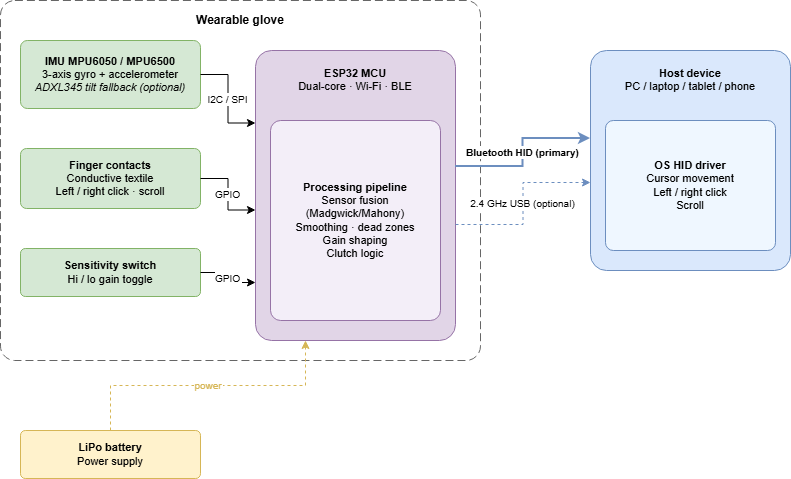
\includegraphics[width=\textwidth]{img/architectural_final.drawio.png}
%     \caption{High-level IoT architecture of the AirGlove system}
%     \label{fig:high_level_iot_architecture}
% \end{figure}